\documentclass[10 pt,usenames,dvipsnames, oneside]{article}
\usepackage{../../modelo-fracoes}
\graphicspath{{../../../Figuras/licao02}}


\begin{document}

\begin{center}
  \begin{minipage}[l]{3cm}
\includegraphics[width=2cm]{../../../Figuras/logo}       
\end{minipage}\hfill
\begin{minipage}[r]{.8\textwidth}
 {\Large \scshape Atividade: Dois chocolates para três irmãs}  
\end{minipage}
\end{center}
\vspace{.2cm}

\ifdefined\prof
\begin{goals}
\begin{enumerate}

\item Reconhecer a necessidade de apresentar uma expressão verbal que identifique a quantidade correspondente à junção de duas ou mais partes correspondentes às frações unitárias de mesmo denominador.

\item Compreender e usar as expressões ``dois terços'', ``três terços'' e ``quatro terços'' como forma de registrar as duas, três ou quatro partes de uma equipartição da unidade em três partes.

\end{enumerate}
\tcblower

\begin{itemize} %s
   \item Recomenda-se que a atividade seja desenvolvida em grupos de 3 a 5 alunos.
   \item Nesta atividade, é importante que os alunos possam ter cópias de figuras ilustrativas das barras de chocolate para dividir e poder avaliar e decidir as suas respostas. Faça cópias das páginas para reprodução.
   \item A opção por um problema de divisão em partes iguais (dois terços corresponde ao resultado da divisão de 2 unidades em 3 partes iguais) no lugar da abordagem ``parte-todo'' (dois terços corresponde a duas partes da equipartição da unidade em três partes) que, no Brasil, costuma ser o mais tradicional, tem duas justificativas: (1) manter a abordagem que marca a lição anterior: equipartição (agora com múltiplas cópias da unidade); (2) amparar a compreensão de frações cujo numerador é maior do que o denominador pela reunião de cópias de partes da unidade (uma vez que pode não parecer coerente nomear uma parte ``maior do que o todo'').
   \item As diversas soluções apresentadas pelos diferentes grupos devem ser discutidas com a turma inteira.
   \item É possível que os alunos utilizem expressões variadas para nomear as partes dos chocolates em cada divisão e para a quantidade de chocolate que cada irmão recebeu. Por exemplo, ``dois dos seis pedaços'', ``dois pedaços de um terço de chocolate''. É importante que a discussão conduza os alunos ao uso de terços:       ``dois terços'', ``quatro terços'', ``seis terços'', etc. Observa-se que o uso de ``sextos'' muito provavelmente indica uma confusão do aluno em relação ao reconhecimento da unidade.
  
\end{itemize} %s


\end{goals}

\bigskip
\begin{center}
{\large \scshape Atividade}
\end{center}
\fi

O pai de Ana, Beatriz e Clara trouxe duas barras de chocolate para serem repartidas entre elas.

\begin{center}
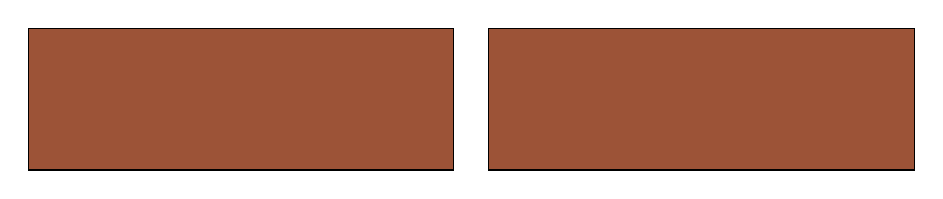
\begin{tikzpicture}[x=1mm,y=1mm, scale=0.9]
\draw[fill=Sepia!60] (0,0) rectangle (60,20);
\draw[fill=Sepia!60, shift={(65,0)}] (0,0) rectangle (60,20);
\end{tikzpicture}
\end{center}

Ana propôs que cada barra fosse dividida em três partes iguais e que cada irmã ficasse com duas dessas partes.

\begin{center}
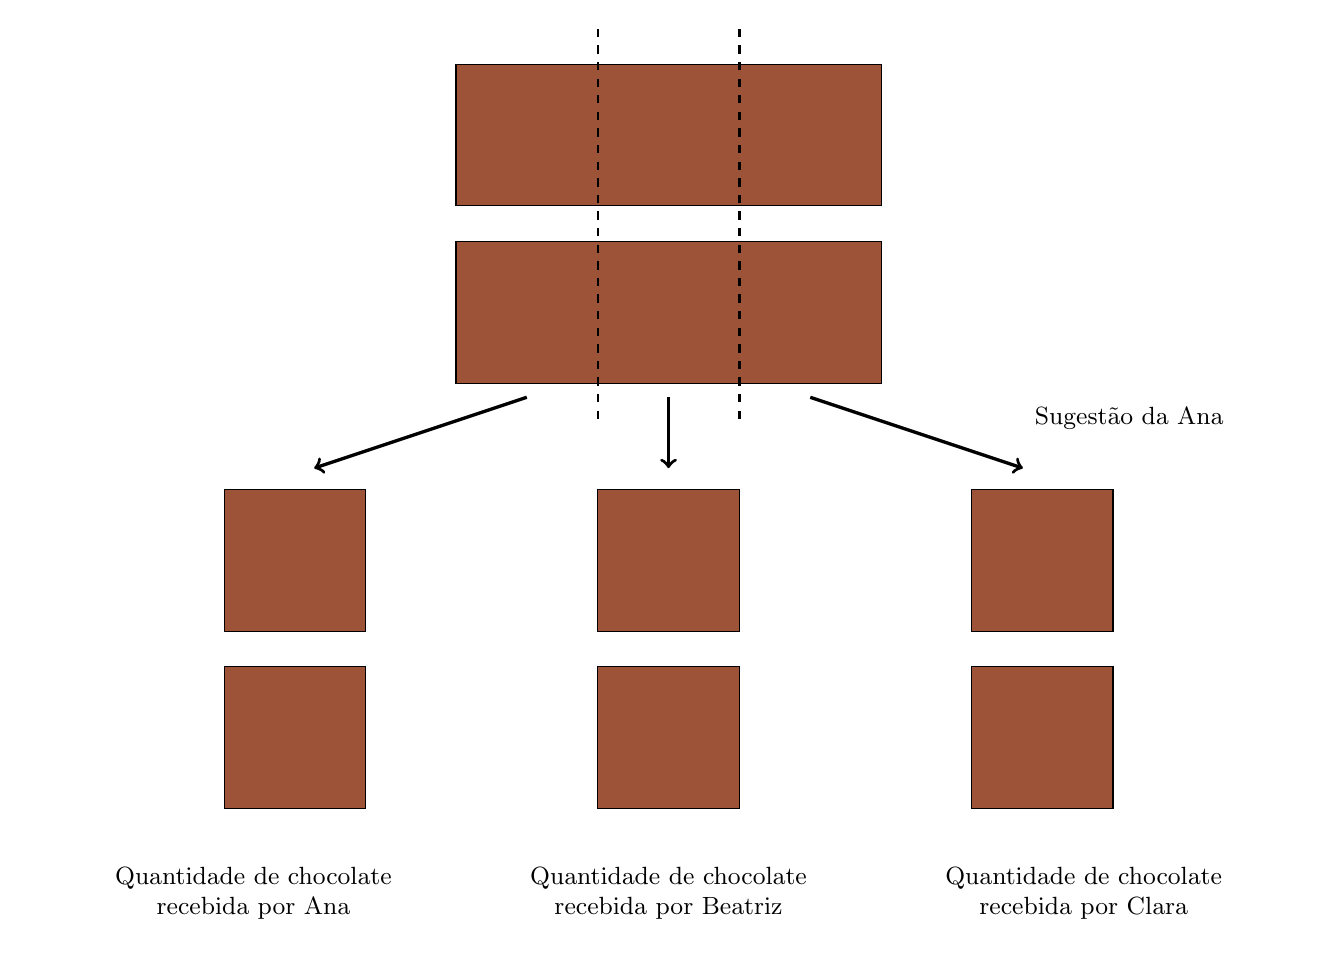
\begin{tikzpicture}[x=1mm,y=1mm,scale=0.9]
%%%%%%%%%% espaço entre um início de barra repartida e outro.
\def\hsp{150} 
%%%%%%%%%% barras de chocolate
\draw[fill=Sepia!60](0,10) rectangle (60,30);
\draw[fill=Sepia!60] (0,-15) rectangle (60,5);

%%%%%%%%% cortes
\draw[dashed, thick] (20,35) -- (20,-20);
\draw[dashed, thick] (40,35) -- (40,-20);

%%%%%%%%% setas
\draw[very thick, ->] (10,-17) -- (-20,-27);
\draw[very thick, ->] (30,-17) -- (30,-27);
\draw[very thick, ->] (50,-17) -- (80,-27);

\node at (95,-20) {\parbox[b]{30mm}{\centering  \small Sugestão da Ana}};

%%%%%%%%%%%%%%%%%%Pedaços repartidos  
\draw[fill=Sepia!60,xshift=-\hsp] (20,-50) rectangle (40,-30);
\draw[fill=Sepia!60,xshift=-\hsp] (20,-75) rectangle (40,-55);

\draw[fill=Sepia!60] (20,-50) rectangle (40,-30);
\draw[fill=Sepia!60] (20,-75) rectangle (40,-55);

\draw[fill=Sepia!60,xshift=\hsp] (20,-50) rectangle (40,-30);
\draw[fill=Sepia!60,xshift=\hsp] (20,-75) rectangle (40,-55);

%%%%%%%%% Texto embaixo
% \draw [thick, decoration={brace,mirror,raise=5}, decorate, xshift=-\hsp] (31.25,-2) -- (51.25,-2) node [pos=0.5,anchor=north,yshift=-10] {\parbox[b]{40mm}{\centering Quantidade de chocolate recebida por Ana}};

\node [xshift=-\hsp] at (30,-87) {\parbox[b]{55mm}{\centering \small Quantidade de chocolate \\ recebida por Ana}};

\node at (30,-87) {\parbox[b]{55mm}{\centering  \small Quantidade de chocolate \\ recebida por Beatriz}};

\node  [xshift=\hsp] at (30,-87) {\parbox[b]{55mm}{\centering  \small Quantidade de chocolate \\ recebida por Clara}};

%%%%%%%%%%%% Balões em volta
% \draw [dotted, xshift=-\hsp] (30,-52.5) ellipse (20mm and 30mm);
% \draw [dotted] (30,-52.5) ellipse (20mm and 30mm);
% \draw [dotted, xshift=\hsp] (30,-52.5) ellipse (20mm and 30mm);
\end{tikzpicture}
\end{center}

\begin{enumerate}[label=\alph*)] %s
  \item Na divisão de cada uma das barras de chocolate em três partes iguais, cada parte é que fração de uma barra de chocolate?
  \item Você concorda com a divisão que Ana sugeriu? Explique.
  \item Com essa divisão, as três irmãs receberam a mesma quantidade de chocolate?
  \item Na divisão proposta por Ana, como você nomearia, usando fração de uma barra de chocolate, a quantidade de chocolate que cada irmã recebeu?
\end{enumerate}

Ana não quer o chocolate e decidiu dar a quantidade de chocolate que recebeu na divisão das barras para as suas irmãs.

\begin{enumerate}[label=\alph*)]
\setcounter{enumi}{4}
\item Se Ana desse metade da quantidade de chocolate que recebeu para cada uma de suas irmãs, que quantidade de chocolate Beatriz e Clara passariam a ter? Como você nomearia, usando frações, essas quantidades?
\item E se Ana desse toda a quantidade de chocolate que recebeu para Beatriz, que quantidade de chocolate  Beatriz passaria a ter? Como você nomearia, usando frações, essa quantidade?
\end{enumerate} %s

\ifdefined\prof
\clearpage
\begin{solucao}

\begin{enumerate} [label=\alph*)] %d
    \item  Um terço.
    \item  Sim, pois a divisão foi justa no sentido de cada irmã ter recebido a mesma quantidade de chocolate.
    \item  Sim, pois cada irmã recebeu dois pedaços que equivalem, cada um, a um terço de uma barra de chocolate.
    \item  Dois terços de uma barra.
    \item  Três terços de uma barra, ou seja, uma barra inteira de chocolate.
    \item  Quatro terços de uma barra, ou seja, uma barra inteira e um terço de chocolate.
\end{enumerate} %d

\end{solucao}
\fi

\end{document}